\section{General resource fragments}
\label{sec:frag}

State convertibility within a given resource theory is often a hard question to address due to the intricate structure of the theory.
In general, the structure of a theory $\R$ is described by a pre-order $\prec_\R$ \nick{expand / move to intro}.
Subdividing magic theories into $\sigma$-fragments \nick{helps}.
\subsection{Monotones}\label{sec:mono}

Resource theories are commonly equipped with monotones which quantify the resource\nick{CITE}. 
\begin{definition}[\textbf{Resource monotone}]\label{def:mono}
    Let $\R = (\F, \O)$ be a general resource theory.
    A monotone $\M$ is a projection from the set of all states of the theory to the real line, satisfying two conditions:
    \begin{enumerate}
        \item All free states are mapped onto 0, $\M(\sigma) = 0,\ \sigma \in \F$;
        \item $\M$ is monotonically decreasing under free operations, $\M(\rho_1) \leq \M(\rho_2)$ whenever $\rho_1 \prec_{\R} \rho_2$.
    \end{enumerate}
\end{definition}
The first condition reflects the property that all free states can be converted into each other, hence they need to be mapped onto the same number, by convention 0.
The second condition reflects the no resource generating property of free operations, thus monotones respect the pre-order $\prec_\R$ of the theory.
Furthermore, if a monotone satisfies the additivity condition,
\begin{equation}
    \M(\rho_1 \otimes \rho_2) = \M(\rho_1) + \M(\rho_2),
\end{equation}
it is of practical importance for resource distillation, which we discuss in~\cref{sec:distill} within the context of magic.

A very commonly used magic monotone is the \emph{mana} of a state \nick{CITE}, defined as
\begin{equation}
    \mana{\rho} \coloneqq \log{\left(\sum\limits_{\bmz \in \pd} \abs{\W[\bmz]{\rho}}\right)}.
\end{equation}
It is a monotone, additive function of the $\ell_1$-norm of negativity~\nick{CITE}.

\subsection{Fragments}

Monotones reduce the structure of the resource theory $\R$ into a real number ordering.
Therefore, two states, even if incomparable in $\R$, are always mapped onto ordered real numbers.
This is a generic approach that ensures a form of state comparison and resource quantification.
However, motivated by $\sigma$-fragments in magic theories, it is clear that we can often reduce the theory by a less \nick{information-collapsing} projection into a subtheory $\R'$ which has a tractable pre-order $\R'$, as sketched in~\cref{fig:fragments}.
\begin{figure}[t]
    \centering
    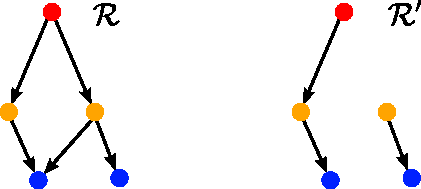
\includegraphics[height=3cm]{sections/major/fragments.pdf}
    \caption{Fragments \nick{Split into subfigures}
    }
    \label{fig:fragments}
\end{figure}
We define such a resource projection for general resource theories as follows.
\begin{definition}[\textbf{Resource projection}]\label{def:fragment}
    Let a resource theory $\R = (\F, \O)$ have pre-order $\prec_{\R}$ and operational composition rule $\circ_{\R}$. 
    Any subtheory $\R' = (\F', \O')$ with pre-order $\prec_{\R'}$ and operational composition rule $\circ_{\R'}$ is called a resource fragment iff there exists a surjective projection $\Pi \equiv (\Pis, \Pio): \R \mapsto \R'$ that satisfies the following two conditions.
    \begin{enumerate}
        \item $\Pis: \cal{B}(\cal{H}) \mapsto \cal{B}(\cal{H})$ and $\Pis(\rho_2) \nprec_{\R'} \Pis(\rho_1)$ whenever $\rho_1 \prec_{\R} \rho_2$;
        \item $\Pio: \O \mapsto \O'$ and $\Pio(\E_1) \circ_{\R'} \Pio(\E_2) = \Pio(\E_1 \circ_{\R} \E_2)$ for all free operations $\E_1, \E_2 \in \O$.
    \end{enumerate}
    We call $\Pi$ a resource projection.
\end{definition}
Fragment $\R'$ is the image of the projection $\Pi$.
Considering a resource projection is particularly useful when the pre-order of the fragment is tractable.
Note the subtle difference of condition 1 in~\cref{def:fragment} and condition 2 in~\cref{def:mono}, which is due to fragments generally retaining a pre-order, while monotones impose a total order.

A monotone is the projection with the simplest tractable order as formally stated in~\cref{thm:monofrag}.
\begin{proposition}\label{thm:monofrag}
	Let $\M$ be a resource monotone of a resource theory $\R$. 
	Then $\M$ is a resource projection that reduces the pre-order $\prec_\R$ to a total order.
\end{proposition}
\begin{proof}
	Consider a monotone $\M$ in the context of a general resource theory $\R = (\F, \O)$.
	Let $\R' = (\F', \O')$, where $\F' \equiv \{0\}$ and $\O'$ is the set of non-increasing real functions mapping the set of non-negative real numbers $\mathbb{R}_{\geq 0}$ to itself. 
	We also set $\prec_{\R'}$ as the usual total order $\leq$ and $\circ_{\R'}$ as the composition of real functions.
	
	Let $\Pis = \M$.
	The defining properties of a monotone, given in~\cref{def:mono}, ensure condition 1 of~\cref{def:fragment}.
	
	Let $\Pio$ project any $\E \in \O$ onto a function $f \in \O$ which maps $\M(\rho)$ onto $\M(\E(\rho))$ for all states $\rho$.
	
	The ordered pair $(\Pis, \Pio)$ is the resource projection which corresponds to monotone $\M$.
\end{proof}

We now justify the name $\sigma$-fragment for the subdivision of a magic theory $\R = (\F, \O)$, by establishing a resource projection which reduces $\R$ into any subtheory $(\F, \O_\sigma)$.
\begin{proposition}
    Let $\R = (\F, \O)$ be a theory of magic.
    Every $\sigma$-fragment $(\F, \O_\sigma)$ is a resource fragment of $\R$.
\end{proposition}
\begin{proof}
    Let the state projection be the identity projection $\Pis:\F\mapsto\F$.
    
    Consider the operation projection $\Pio:\O \mapsto \O_\sigma$, defined as
    \begin{equation}
    \Pio(\E) =
    \begin{cases}
        \E,\ &\sigma \in \O, \\
        1_{\rm{C}},\ &\sigma \notin \O.
    \end{cases}
    \end{equation}
    The ordered pair $(\Pis, \Pio)$ acts as the desired projection.
\end{proof}

An important example of a fragment appears in quantum thermodynamics. 
Consider a projection $\Pi$, such that $\Pis$ dephases all states in the energy eigenbasis, while $\Pio$ maps all free operations to themselves.
Then $\Pi$ describes the theory in the absence of coherences and the new pre-order is simply thermo-majorization, which in fact is fully solvable in the form of entropic conditions~\cite{cit:gour}. \nick{expand/rephrase}

Existing magic theories can be thought of as fragments of $\Rmax$.
\begin{proposition}
    Every theory of magic $\R$ is a fragment of the maximal theory $\Rmax$.
\end{proposition}
\begin{proof}
    Consider the state projection $\Pis:\Fmax \mapsto \F$, defined as
    \begin{equation}
    \Pis(\sigma) =
    \begin{cases}
        \sigma,\ &\sigma \in \F, \\
        \frac{1}{d}\id,\ &\sigma \notin \F.
    \end{cases}
    \end{equation}
    \nick{Perhaps $\Pis = $ identity}
    Let $1_{\rm{C}}$ denote the identity channel.
    Consider the operation projection $\Pio:\Omax \mapsto \O$, defined as
    \begin{equation}
    \Pio(\E) =
    \begin{cases}
        \E,\ &\sigma \in \O, \\
        1_{\rm{C}},\ &\sigma \notin \O.
    \end{cases}
    \end{equation}
    The orderd pair $(\Pis, \Pio)$ acts as the desired projection.
\end{proof}